\documentclass{article}
\usepackage[final]{neurips_2020}
\usepackage[utf8]{inputenc}
\usepackage[T1]{fontenc}    % use 8-bit T1 fonts
\usepackage{hyperref}       % hyperlinks
\usepackage{url}            % simple URL typesetting
\usepackage{booktabs}       % professional-quality tables
\usepackage{amsfonts}       % blackboard math symbols
\usepackage{nicefrac}       % compact symbols for 1/2, etc.
\usepackage{microtype}      % microtypography
\usepackage{amsthm}
\usepackage{amssymb}
\usepackage{amsmath}
\usepackage{bbm}
\usepackage{algorithm}
\usepackage{algpseudocode}
\usepackage{graphicx}
% \graphicspath{ {./images/} }

\newcommand{\EX}[0]{\mathbb{E}} % expected value
\newcommand{\V}[0]{\mathbb{V}}
\newcommand{\IF}[2]{\mathbbm{1}_{#1}(#2)} % indicator function
\renewcommand{\vec}[1]{\mathbf{#1}}

\title{20592 - Statistics and Probability\\Bayesian Estimation of a Probit Regression Model}
\author{%
  Stefano Cortinovis \\
  \texttt{stefano.cortinovis@studbocconi.it}
  \And
  Daniele Micheletti\\
  \texttt{daniele.micheletti@studbocconi.it}
  \And
  Andrea Teruzzi\\
  \texttt{andrea.teruzzi@studbocconi.it}
  \And
  Leonardo Yang\\
  \texttt{leonardo.yang@studbocconi.it}
}

\begin{document}

\maketitle

\section{Project Introduction}

This report aims at illustrating the use of Bayesian methods for estimating the coefficient of a probit regression model for binary outcomes. Section 2 succinctly describes the probit regression model and the Bayesian approach to estimating its coefficients using instances of the Metropolis-Hastings algorithm. Next, section 3 and 4 briefly explain two such instances, namely the Metropolis algorithm and the auxiliary variable Gibbs sampler. Then, section 5 compares the performance of the two algorithms on a dataset provided by Finney \cite{finney1947estimation} to study the relationship between the occurrence of transient skin vasorestriction and the rate and volume of the air inspired by the individuals undergoing the test. Performance is assessed by means of basic diagnostics, such as trace plots and acceptance rate computation. As prescribed by the project's description, this report is heavily inspired by Albert and Chib \cite{albert1993bayesian}.

\section{Probit Model}
Let \(Y_1,...,Y_n\) be a sample of \(n\) independent binary random variables, where \(Y_i \sim B(p_i)\). The probit model assumes that \(p_i = \Phi(\vec{x}_i^T \beta), i = 1,....,n\), where \(\vec{x}_i^T = \begin{pmatrix} x_{i1} & \hdots & x_{1k} \end{pmatrix}\) is a \(k\)-dimensional vector of observed covariates, \(\beta\) is a \(k \times 1\) vector of unknown coefficients, and \(\Phi\) denotes the cumulative distribution function of a standard normal random variable. Given a sample of observations \(\{(y_i, \vec{x}_i)\}_{i=1}^n\), the standard estimation procedure for the probit model employs the maximum likelihood estimation of coefficient \(\beta\). However, the Bayesian approach to the estimation of \(\beta\) constitutes an interesting alternative. In particular, suppose the posterior density of \(\beta\), denoted by \(\pi(\beta|\vec{y})\),  was known and tractable. Then, the value of the posterior first moment, \(\EX[\beta|\vec{y}]\), would constitute a reasonable estimate for \(\beta\). However, if we denote the proper or improper prior density of \(\beta\) by \(\pi(\beta)\), the posterior density of \(\beta\) has the form:
\begin{equation*}
    \pi(\beta|\vec{y}) \propto \pi(\beta) \prod_{i=1}^n \Phi(\vec{x}_i^T \beta)^{y_i} (1 - \Phi(\vec{x}_i^T \beta))^{1 - y_i},
\end{equation*}
which is intractable.
\par 
To address the issue of sampling from intractable posteriors, the Metropolis-Hastings algorithm is often employed in Bayesian statistics. By means of a proposal density used to sample candidates and a probabilistic criterion to accept or reject them, this method is able to generate a Markov chain \(\{\beta_t\}_{t \geq 1}\) having the target posterior as stationary distribution. This means that, if such a Markov chain of length \(T\) is generated and \(t_0 < T\) denotes the step at which the chain can be considered to have converged to the stationary distribution \(\pi({\beta|\vec{y}})\), the estimator
\begin{equation*}
    \hat{\beta} = \frac{1}{T-t_0} \sum_{t=t_0}^T \beta_t
\end{equation*}
is unbiased and consistent for \(\EX[\beta|\vec{y}]\).
\par
Instances of the MH algorithm differ in terms of the proposal density used. In particular, the methods employed in this report are the Metropolis algorithm and the auxiliary variable Gibbs sampler.

\section{Metropolis Algorithm}
The Metropolis algorithm is an instance of the MH algorithm with proposal density \(q(\beta^*|\beta_t)\) symmetric around the current value of the chain, namely \(\beta_t\). When \(q(y|x)\) has such a property, the candidate acceptance probability becomes:
\begin{equation*}
    \alpha(\beta_t, \beta^*) = \min\Bigg\{1, \frac{\pi(\beta^*|\vec{y})}{\pi(\beta_t|\vec{y})}\Bigg\} = \min\Bigg\{1, \frac{\pi(\beta^*)}{\pi(\beta_t)}\frac{\mathcal{L}(\beta^*)}{\mathcal{L}(\beta_t)}\Bigg\}
\end{equation*}
where \(\mathcal{L}(\beta)\) denotes the likelihood of the model at \(\beta\).
\par
The proposal used in this report is a multivariate normal distribution. In particular, at each sampling step performed by the algorithm, a candidate is drawn from \(q(\beta^*|\beta_t) = N_k(\beta_t,V)\) where \(V = \mathcal{I}^{-1}(\beta_t)\) is the inverse of the Fisher information matrix computed at the current value of \(\beta_t\). Moreover, recall that, in the case of a generalized linear model with link function \(g\), it can be shown that \(\mathcal{I}(\beta_t) = X^T W X\) where \(X = \begin{bmatrix} \vec{x}_1 \hdots \vec{x}_n \end{bmatrix}\) and \(W\) is a diagonal matrix such that 
\begin{equation*}
    w_{ii} = \frac{1}{\V(Y_i)}\bigg(\frac{\partial \vec{x}_i^T \beta}{\partial g(\vec{x}_i^T \beta)}\bigg)^{-2}.
\end{equation*}
This means that, in the case of the probit model, \(w_{ii} = \phi^2(\vec{x}_i^T \beta)/(p_i(1 - p_i))\).
\par 
Algorithm \ref{metropolis} summarizes the steps performed by the Metropolis algorithm presented in this section.

\begin{algorithm}
\caption{Metropolis Algorithm for Probit Estimation}\label{metropolis}
\begin{algorithmic}[1]
\Procedure{Metropolis}{$\beta_0$}
    \State $\beta \gets \beta_0$
    \State $m \gets [\beta_0]$
    \Repeat
        \State $\beta^* \gets \beta^* \sim N_k(\beta,\mathcal{I}^{-1}(\beta))$
        \State $u \gets U \sim \text{Unif}(0, 1)$
        \State $\alpha \gets \alpha(\beta, \beta^*) = \min\big\{1, \frac{\pi(\beta^*)}{\pi(\beta)}\frac{\mathcal{L}(\beta^*)}{\mathcal{L}(\beta)}\big\}$
        \If{$u \leq \alpha$}
            \State $\beta \gets \beta^*$
        \EndIf
        \State \textbf{append} $\beta$ to $m$
    \Until {stopping criterion is reached}
    \State \textbf{return} $m$
\EndProcedure
\end{algorithmic}
\end{algorithm}


\section{Auxiliary Variable Gibbs Sampler}
Sometimes, when a Gibbs sampler cannot be easily devised for a target distribution, it is possible to exploit a vector of auxiliary random variables to successfully complete the task. This straightforward extension of the simple Gibbs sampler is called auxiliary variable Gibbs sampler. In particular, if the target distribution is \(\pi(\beta|\vec{y})\) and we are able to find a random vector \(\vec{Z}\) such that the full conditionals \(\pi(\beta|\vec{y}, \vec{Z})\) and \(\pi(\vec{Z}|\vec{y}, \beta)\) are known and can be sampled from, then a Gibbs sampler can be used to generate the Markov chain \(\{(\beta_t, \vec{Z}_t)\}_{t\geq 1}\). Crucially, it is possible to show that the sequence \(\{\beta_t\}_{t\geq 1}\) is also a Markov chain and has the target distribution \(\pi(\beta|\vec{y})\) as its stationary distribution. 
\par
In regards to the scenario considered in this report, it turns out that any probit model can be expressed in terms of a normal linear model. In particular, introduce auxiliary vector \(\vec{Z} = \begin{pmatrix} Z_1 \hdots Z_n \end{pmatrix}\) such that the \(Z_i\) are independent \(N(\vec{x}_i^T \beta, 1)\) and define \(Y_i = \IF{(0, \infty)}{Z_i}\), i.e. \(Y_i = 1\) if \(Z_i > 0\) and \(Y_i = 0\) otherwise. Then, it is possible to show that the \(Y_i\) are independent Bernoulli random variables with \(p_i = \Phi(\vec{x}_i^T\beta)\), as prescribed by the probit model. 
\par 
As mentioned above, to use a Gibbs sampler to sample from target \(\pi(\beta|\vec{y})\) using \(\vec{Z}\) as the auxiliary variable, the full conditionals \(\pi(\beta|\vec{y}, \vec{Z})\) and \(\pi(\vec{Z}|\vec{y}, \beta)\) have to be known distributions. First, the full conditional of \(\beta\) is given by:
\begin{equation*}
    \pi(\beta|\vec{y}, \vec{Z}) = \pi(\beta|\vec{Z}) \propto \pi(\beta) \pi(\vec{Z}|\beta) = \pi(\beta) \prod_{i=1}^n\phi(Z_i;\vec{x}_i^T \beta, 1),
\end{equation*}
which depends on the choice of the prior \(\pi(\beta)\). In particular, if \(\pi(\beta)\) is chosen to be non-informative, we have that
\begin{align*}
    \pi(\beta|\vec{y}, \vec{Z}) &\propto \prod_{i=1}^n\phi(Z_i;\vec{x}_i^T \beta, 1) \propto \exp\Bigg\{\sum_{i=1}^n (Z_i - \vec{x}_i^T \beta)^2\Bigg\} \\
                                &\propto \exp\Big\{(\vec{X} \beta)^T (\vec{X} \beta) - 2 (\vec{X}\beta)^T \vec{Z}\Big\} \\
                                &= \exp\Big\{(\vec{X} \beta)^T (\vec{X} \beta) - 2 (\vec{X}\beta)^T 
                                \vec{X} (\vec{X}^T \vec{X})^{-1}\vec{X}^T \vec{Z}\Big\}.
\end{align*}
By completing the square with the product of the transpose of \(\vec{X} (\vec{X}^T \vec{X})^{-1}\vec{X}^T \vec{Z}\) with itself,
\begin{align*}
    \pi(\beta|\vec{y}, \vec{Z}) &\propto \exp\Big\{\big(\vec{X}\beta - \vec{X} (\vec{X}^T \vec{X})^{-1}\vec{X}^T \vec{Z}\big)^T\big(\vec{X}\beta - \vec{X} (\vec{X}^T \vec{X})^{-1}\vec{X}^T \vec{Z}\big)\Big\} \\
    &= \exp\Big\{\big(\beta - (\vec{X}^T \vec{X})^{-1}\vec{X}^T \vec{Z}\big)^T (X^T X) \big(\beta - (\vec{X}^T \vec{X})^{-1}\vec{X}^T \vec{Z}\big)\Big\}
\end{align*}
which is the kernel of a multivariate normal random variable with with mean \(\hat{\beta}_Z = (\vec{X}^T \vec{X})^{-1}\vec{X}^T \vec{Z}\) and variance \((\vec{X}^T \vec{X})^{-1}\). That is, if \(\pi(\beta)\) is chosen to be non-informative, \(\beta|\vec{y}, \vec{Z} \sim N_k(\hat{\beta}_Z, (\vec{X}^T\vec{X})^{-1})\). On the other hand, if the conjugate prior \(\beta \sim N_k(\beta^*, \vec{B}^*)\) is chosen, we it can be shown that \(\beta | \vec{y}, \vec{Z} \sim N_k(\tilde{\beta}, \tilde{\vec{B}})\) where \(\tilde{\beta} = (\vec{B}^{*-1} + \vec{X}^T\vec{X})^{-1}(\vec{B}^{*-1}\beta^* + \vec{X}^T\vec{Z})\) and \(\tilde{\vec{B}} = (\vec{B}^{*-1} + \vec{X}^T\vec{X})^{-1}\). 
\par
Next, for each \(i\), the full conditional of \(Z_i\) is given by:
\begin{equation*}
    \pi(Z_i | \vec{y}, \beta) \propto 
    \begin{cases}
        \phi(Z_i; \vec{x}_i^T \beta, 1) \IF{(0, +\infty)}{Z_i} & \text{if } y_i = 1 \\
        \phi(Z_i; \vec{x}_i^T \beta, 1) \IF{(-\infty, 0]}{Z_i} & \text{if } y_i = 0
    \end{cases}
\end{equation*}
that is, \(Z_i\) has a \(N(\vec{x}_i^T \beta, 1)\) truncated by 0 at the left if \(y_i = 1\) and at the right if \(y_i = 0\).
\par 
Notice that, if we choose the prior \(\pi(\beta)\) in one of the two ways mentioned above, both full conditionals have a known distribution and can be easily sampled from. This means that we can indeed exploit \(\vec{Z}\) to use an auxiliary variable Gibbs sampler to sample from \(\pi(\beta|\vec{y})\). Finally, Algorithm \ref{gibbs} summarizes the steps performed by the auxiliary variable Gibbs sampler presented in this section.

\begin{algorithm}
\caption{Auxiliary Variable Gibbs Sampler for Probit Estimation}\label{gibbs}
\begin{algorithmic}[1]
\Procedure{AuxiliaryGibbs}{$\beta_0$}
    \State $\beta \gets \beta_0$
    \State $m \gets [\beta_0]$
    \Repeat
        \State $\vec{Z} \gets \vec{Z} | \vec{y}, \beta \sim \pi(\vec{Z}|\vec{y}, \beta)$
        \State $\beta \gets \beta | \vec{y}, \vec{Z} \sim \pi(\beta | \vec{y}, \vec{Z})$
        \State \textbf{append} $\beta$ to $m$
    \Until {stopping criterion is reached}
    \State \textbf{return} $m$
\EndProcedure
\end{algorithmic}
\end{algorithm}

\section{Diagnostics and Performance Comparison}
% summary of procedures (test MH and Gibbs on same dataset(Finney47) and use of 2 priors for Gibbs(noninfo and multinorm) and 3 for MH(noninfo, lowvar multinorm, highvar multinorm)).
% % distplot comparison with paper,

Following the pseudo-code described in Algorithm \ref{metropolis} and \ref{gibbs} we implemented the Metropolis and auxiliary variable Gibbs sampler algorithms using the Python programming language. In both cases, the user is allowed to specify whether to include an intercept in the estimation, as well as the initial value for \(\beta_0\), with the default being the OLS estimate for \(\beta\). Moreover, for the Metropolis algorithm, the user is allowed to specify a custom prior distribution, while the Gibbs sampler implemented the full conditional associated with the non-informative and conjugate multivariate normal prior mentioned in Section 4.
\par
What follows is a short summary of the tests performed to assess the performance of the two algorithms. The dataset used for all tests is the one introduced by Finney  \cite{finney1947estimation} and briefly mentioned in Section 1.
\par
In particular, both the Metropolis algorithm and the auxiliary variable Gibbs sampler were used to estimate a probit model using three different priors:
\begin{enumerate}
    \item Non-informative prior; 
    \item Multivariate normal prior with high variance (diagonal covariance matrix with diagonal entries equal to 10) centered around the true values of the betas;
    \item Multivariate normal prior with low variance (diagonal covariance matrix with diagonal entries equal to 1) centered around the true values of the betas.
\end{enumerate}
Every model estimated included the intercept and the starting value \(\beta_0\) was taken to be equal to \(\hat\beta_{OLS} = (\vec{X}^T \vec{X})^{-1}\vec{X}^T \vec{y}\) for every estimation. For both algorithms, and for each of the priors mentioned above, the fitting procedure was run thrice with number of iterations equal to 200, 800, and 20000, respectively. Lastly, a \textit{warmup}, i.e. number of iterations discarded from the output chain before computing the Bayesian estimator \(\hat{\beta}\), of 200 was used for the runs with 20000 total iterations.
\par
Below, distribution and trace plots of \(\beta\) for the simulations performed with 800 iterations are shown. Additionally, the acceptance rate behaviour across iterations for the Metropolis algorithm is also plotted.  
% distplots are different in shape but similar scale, is it good?

% Describe traceplots (Gibbs wiggle wiggle),
% acceptance rate (0.4, not too high(local), not too low(stuck) -> slow convergence to stationary distribution, tao choice)

First, Figure \ref{fig:trace_1} compares the trace plots obtained using the two algorithms with a non-informative prior. From that, we can immediately notice how the Gibbs Sampler trace plot seems to be of higher quality in terms of the final chain's representativeness of the posterior of \(\beta\). The main reason behind this is that, since the Gibbs Sampler can be interpreted of the MH framework as always accepting the proposal, it seems to better explore the sample space of \(\beta\). The Metropolis algorithm, instead, accepts the proposal with a certain probability. This means that, sometimes, the proposal is rejected and the new state of the Markov chain is the same as in the previous iteration. From the trace plot, we can see that the output chain for the Metropolis algorithm explores the sample space of \(\beta\) based on "local movements", making the next observation more likely to be correlated with the previous one and increasing the number of iterations required for the chain to reach its stationary distribution. 

\begin{figure}[htp]
    \centering
    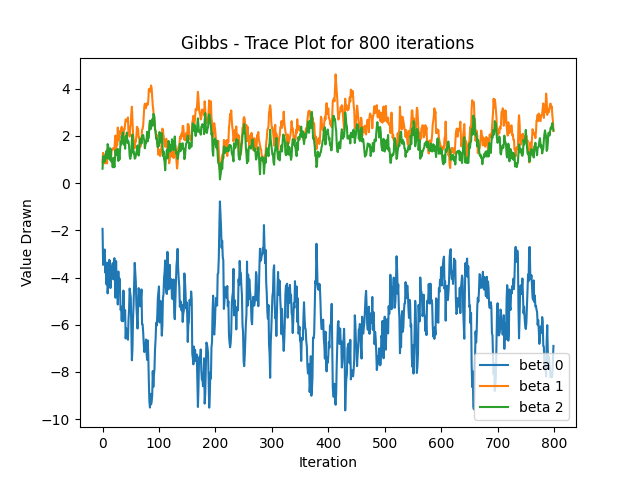
\includegraphics[scale=0.6]{images/trace_gibbs_noinfo_800_warmup_0.png}
    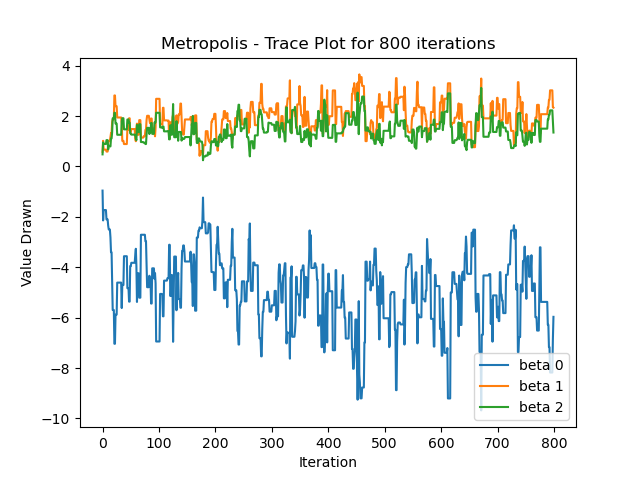
\includegraphics[scale=0.6]{images/trace_metropolis_noinfo_800_warmup_0.png}
    \caption{Trace plots for both algorithms with non informative prior.}
    \label{fig:trace_1}
\end{figure}


% (Therefore, if the aim was to obtain a sample of independent observations we would recommend to perform a systematic random sampling on the output sample.) %makes sense ?)  

Moreover, from the simulations performed using Metropolis, we also noticed that, as shown in Figure \ref{fig:trace_2}, the prior with high variance outperformed the one with low variance. Given that the true value of the coefficients is not very close to zero, this is expected. For priors centered at zero, lower variance means narrower exploration of the sample space of \(\beta\). Regarding the Gibbs Sampler, as shown in figure \ref{fig:trace_3}, the simulation with multivariate normal prior produced a better trace plot then the one with non-informative prior. 

\begin{figure}[htp]
    \centering
    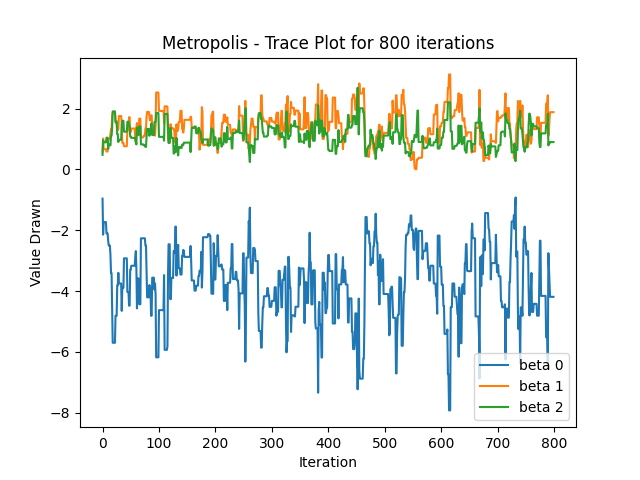
\includegraphics[scale=0.6]{images/trace_metropolis_highvar_800_warmup_0.png}
    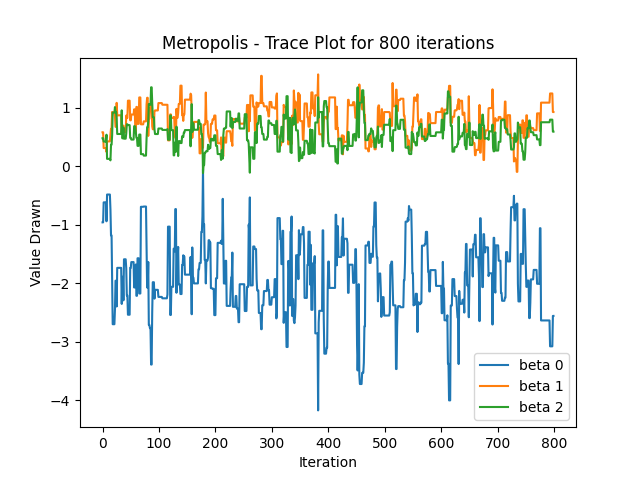
\includegraphics[scale=0.6]{images/trace_metropolis_lowvar_800_warmup_0.png}
    \caption{Starting from the top: trace plot for the coefficients sampled using high variance multivariate normal prior with Metropolis, trace plot for the coefficients sampled using low variance multivariate normal prior with Metropolis.}
    \label{fig:trace_2}
\end{figure}

\begin{figure}[htp]
    \centering
    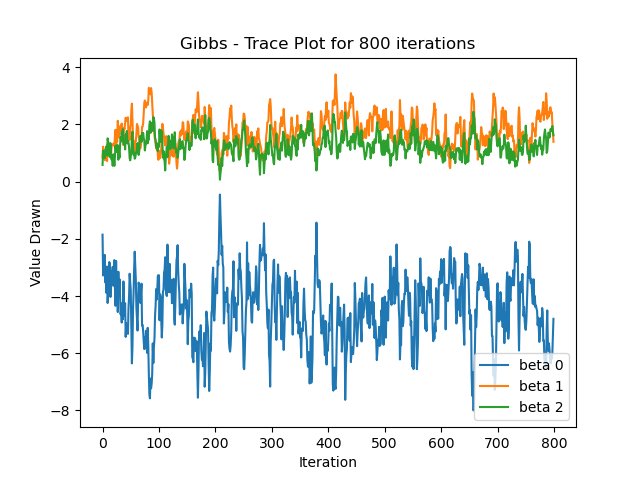
\includegraphics[scale=0.6]{images/trace_gibbs_multinorm_800_warmup_0_high.png}
    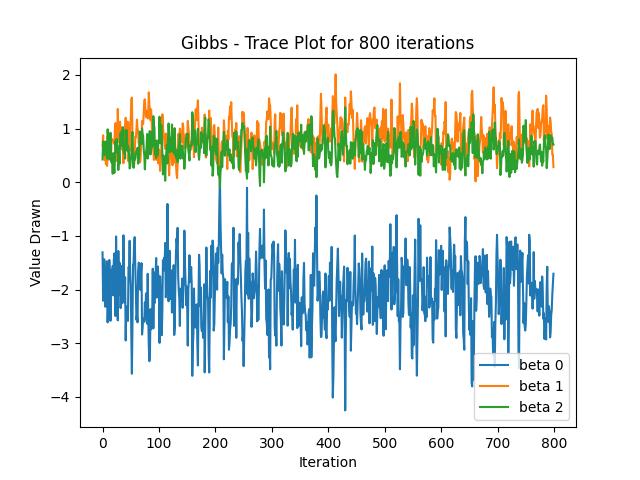
\includegraphics[scale=0.6]{images/trace_gibbs_multinorm_800_warmup_0_low.png}
    \caption{Starting from the top: trace plot for the coefficients sampled using high variance multivariate normal prior on Gibbs, trace plot for the coefficients sampled using low variance multivariate normal prior on Gibbs.}
    \label{fig:trace_3}
\end{figure}
% Firstly, we compared the trace plots. We denote that the Metropolis chain, compared to the Gibbs Sampler one, gets more frequently stuck in certain neighbourhood of the distribution.
% The Gibbs Sampler has a more wiggly shape that guarantees a less local exploration of the distribution of the parameters. 

%add something about the speed to the convergence? Using warmup we skipped this topic

Looking at the acceptance rate of the Metropolis with non-informative prior displayed in Figure \ref{fig:ar}, it is possible to notice a stabilization of the rate around 0.4 after nearly 500 iterations. This value can be considered quite satisfactory. On the one hand, it is not too high, which would lead to the risk of a local exploration. On the other hand, it is not too low, that would lead to the risk of slow convergence to the stationary distribution.

\begin{figure}[htp]
    \centering
    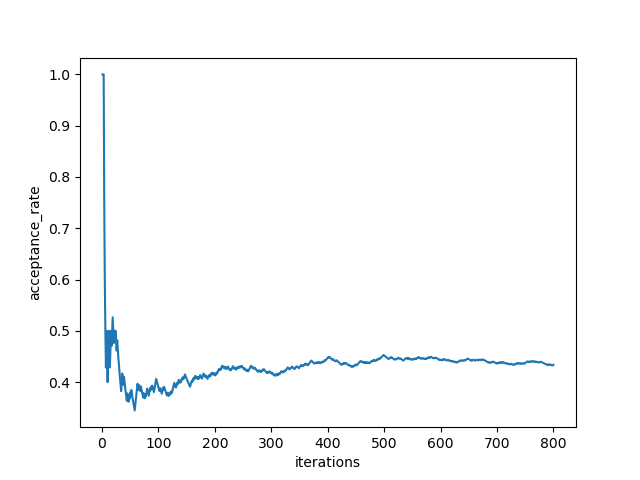
\includegraphics[scale=0.6]{images/ar_metropolis_noinfo_800_warmup_0.png}
    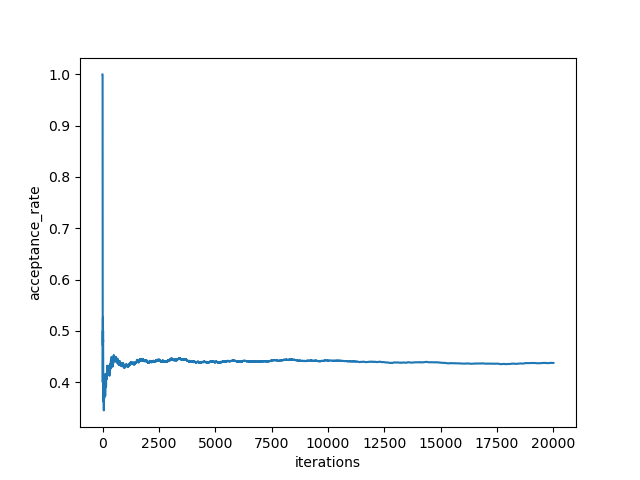
\includegraphics[scale=0.6]{images/ar_metropolis_noinfo_20000_warmup_0.png}
    \caption{Starting from the top: acceptance rate of the Metropolis algorithm with non informative prior for 800 iterations, acceptance rate of the Metropolis algorithm with non informative prior for 20000 iterations.}
    \label{fig:ar}
\end{figure}
Finally the distribution plots of the the parameters obtained, as shown in Figure \ref{fig:dist}, are nearly the same as the ones discussed by Albert and Chib \cite{albert1993bayesian} in their paper. 

\begin{figure}[htp]
    \centering
    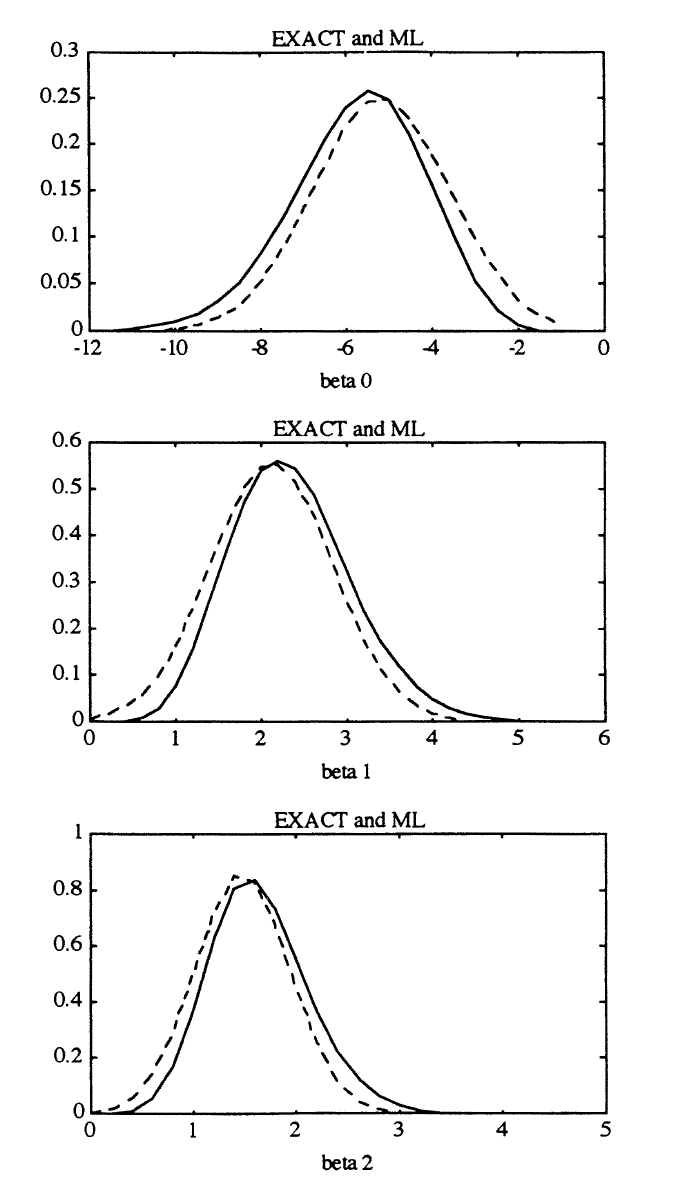
\includegraphics[scale=0.5]{images/albert_chibb.png}
    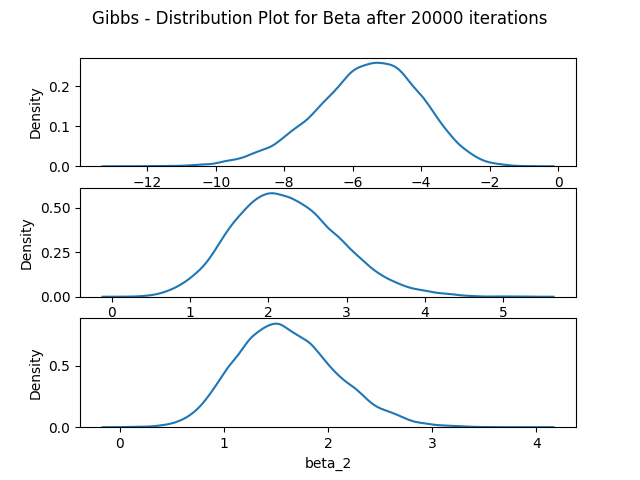
\includegraphics[scale=0.6]{images/dist_gibbs_noinfo_20000_warmup_200.png}
    % 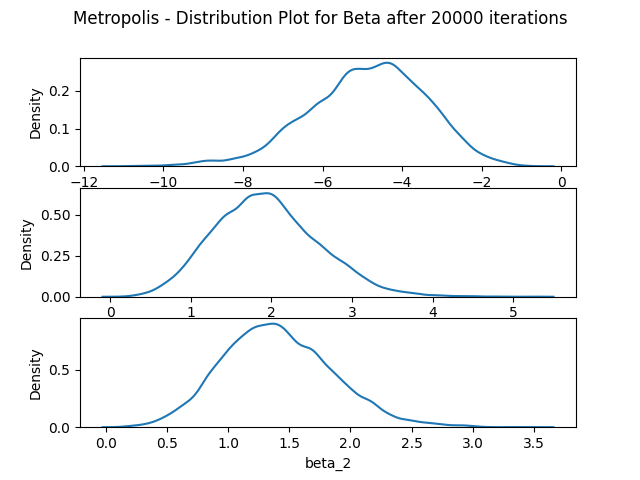
\includegraphics[scale=0.41]{images/dist_metropolis_noinfo_20000_warmup_0.png}
    \caption{Starting from the top: the distribution plots from Albert and Chib, the distribution plots of the parameters with Gibbs and Metropolis, respectively.}
    \label{fig:dist}
\end{figure}

\bibliographystyle{plain}
\bibliography{project}

\end{document}
